\documentclass[twoside]{book}

% Packages required by doxygen
\usepackage{fixltx2e}
\usepackage{calc}
\usepackage{doxygen}
\usepackage[export]{adjustbox} % also loads graphicx
\usepackage{graphicx}
\usepackage[utf8]{inputenc}
\usepackage{makeidx}
\usepackage{multicol}
\usepackage{multirow}
\PassOptionsToPackage{warn}{textcomp}
\usepackage{textcomp}
\usepackage[nointegrals]{wasysym}
\usepackage[table]{xcolor}

% Font selection
\usepackage[T1]{fontenc}
\usepackage[scaled=.90]{helvet}
\usepackage{courier}
\usepackage{amssymb}
\usepackage{sectsty}
\renewcommand{\familydefault}{\sfdefault}
\allsectionsfont{%
  \fontseries{bc}\selectfont%
  \color{darkgray}%
}
\renewcommand{\DoxyLabelFont}{%
  \fontseries{bc}\selectfont%
  \color{darkgray}%
}
\newcommand{\+}{\discretionary{\mbox{\scriptsize$\hookleftarrow$}}{}{}}

% Page & text layout
\usepackage{geometry}
\geometry{%
  a4paper,%
  top=2.5cm,%
  bottom=2.5cm,%
  left=2.5cm,%
  right=2.5cm%
}
\tolerance=750
\hfuzz=15pt
\hbadness=750
\setlength{\emergencystretch}{15pt}
\setlength{\parindent}{0cm}
\setlength{\parskip}{3ex plus 2ex minus 2ex}
\makeatletter
\renewcommand{\paragraph}{%
  \@startsection{paragraph}{4}{0ex}{-1.0ex}{1.0ex}{%
    \normalfont\normalsize\bfseries\SS@parafont%
  }%
}
\renewcommand{\subparagraph}{%
  \@startsection{subparagraph}{5}{0ex}{-1.0ex}{1.0ex}{%
    \normalfont\normalsize\bfseries\SS@subparafont%
  }%
}
\makeatother

% Headers & footers
\usepackage{fancyhdr}
\pagestyle{fancyplain}
\fancyhead[LE]{\fancyplain{}{\bfseries\thepage}}
\fancyhead[CE]{\fancyplain{}{}}
\fancyhead[RE]{\fancyplain{}{\bfseries\leftmark}}
\fancyhead[LO]{\fancyplain{}{\bfseries\rightmark}}
\fancyhead[CO]{\fancyplain{}{}}
\fancyhead[RO]{\fancyplain{}{\bfseries\thepage}}
\fancyfoot[LE]{\fancyplain{}{}}
\fancyfoot[CE]{\fancyplain{}{}}
\fancyfoot[RE]{\fancyplain{}{\bfseries\scriptsize Generated by Doxygen }}
\fancyfoot[LO]{\fancyplain{}{\bfseries\scriptsize Generated by Doxygen }}
\fancyfoot[CO]{\fancyplain{}{}}
\fancyfoot[RO]{\fancyplain{}{}}
\renewcommand{\footrulewidth}{0.4pt}
\renewcommand{\chaptermark}[1]{%
  \markboth{#1}{}%
}
\renewcommand{\sectionmark}[1]{%
  \markright{\thesection\ #1}%
}

% Indices & bibliography
\usepackage{natbib}
\usepackage[titles]{tocloft}
\setcounter{tocdepth}{3}
\setcounter{secnumdepth}{5}
\makeindex

% Hyperlinks (required, but should be loaded last)
\usepackage{ifpdf}
\ifpdf
  \usepackage[pdftex,pagebackref=true]{hyperref}
\else
  \usepackage[ps2pdf,pagebackref=true]{hyperref}
\fi
\hypersetup{%
  colorlinks=true,%
  linkcolor=blue,%
  citecolor=blue,%
  unicode%
}

% Custom commands
\newcommand{\clearemptydoublepage}{%
  \newpage{\pagestyle{empty}\cleardoublepage}%
}

\usepackage{caption}
\captionsetup{labelsep=space,justification=centering,font={bf},singlelinecheck=off,skip=4pt,position=top}

%===== C O N T E N T S =====

\begin{document}

% Titlepage & ToC
\hypersetup{pageanchor=false,
             bookmarksnumbered=true,
             pdfencoding=unicode
            }
\pagenumbering{alph}
\begin{titlepage}
\vspace*{7cm}
\begin{center}%
{\Large rws \\[1ex]\large 0.\+1.\+0 }\\
\vspace*{1cm}
{\large Generated by Doxygen 1.8.13}\\
\end{center}
\end{titlepage}
\clearemptydoublepage
\pagenumbering{roman}
\tableofcontents
\clearemptydoublepage
\pagenumbering{arabic}
\hypersetup{pageanchor=true}

%--- Begin generated contents ---
\chapter{Reader-\/\+Writers Example}
\label{index}\hypertarget{index}{}\hypertarget{index_intro}{}\section{Introduction}\label{index_intro}
An implementation example for reader-\/writers protocol, giving priority to readers.

The goal of this example is to
\begin{DoxyItemize}
\item create two or more readers,
\item create a writer
\item simlutate some reads and some writes on shared data following the reader-\/writers protol.
\end{DoxyItemize}

See \hyperlink{rws_8c_abf9e6b7e6f15df4b525a2e7705ba3089}{main } function to run the code.

\begin{DoxyDate}{Date}
06/05/2018 
\end{DoxyDate}
\begin{DoxyVersion}{Version}
0.\+1.\+0 
\end{DoxyVersion}
\begin{DoxyAuthor}{Author}
Luca Parolari 
\end{DoxyAuthor}

\chapter{File Index}
\section{File List}
Here is a list of all documented files with brief descriptions\+:\begin{DoxyCompactList}
\item\contentsline{section}{\hyperlink{read__and__skip_8c}{read\+\_\+and\+\_\+skip.\+c} \\*Main file }{\pageref{read__and__skip_8c}}{}
\end{DoxyCompactList}

\chapter{File Documentation}
\hypertarget{rws_8c}{}\section{rws.\+c File Reference}
\label{rws_8c}\index{rws.\+c@{rws.\+c}}


Main file.  


{\ttfamily \#include $<$semaphore.\+h$>$}\newline
{\ttfamily \#include $<$pthread.\+h$>$}\newline
{\ttfamily \#include $<$stdio.\+h$>$}\newline
{\ttfamily \#include $<$unistd.\+h$>$}\newline
{\ttfamily \#include $<$stdlib.\+h$>$}\newline
Include dependency graph for rws.\+c\+:
\nopagebreak
\begin{figure}[H]
\begin{center}
\leavevmode
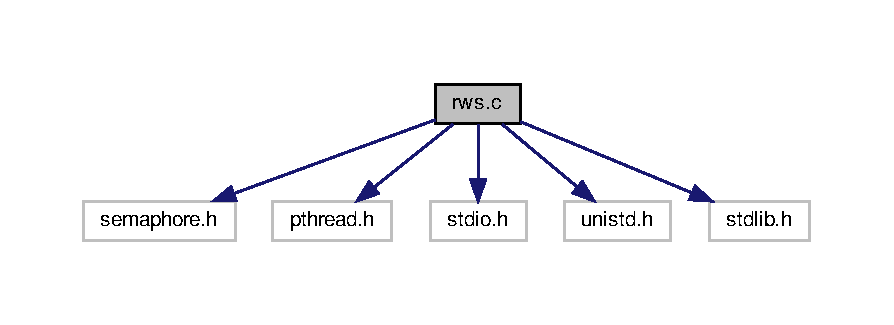
\includegraphics[width=350pt]{rws_8c__incl}
\end{center}
\end{figure}
\subsection*{Functions}
\begin{DoxyCompactItemize}
\item 
void $\ast$ \hyperlink{rws_8c_a9901212efa6943de07eee8a84bb97a61}{reader} (void $\ast$arg)
\begin{DoxyCompactList}\small\item\em Simulates a read procedure. \end{DoxyCompactList}\item 
void \hyperlink{rws_8c_ae4c2d4b7fa17edbf003c6eb85cc9ffe9}{reader\+\_\+internal} (int r)
\begin{DoxyCompactList}\small\item\em Executes a read. \end{DoxyCompactList}\item 
void $\ast$ \hyperlink{rws_8c_a35c056ce555ff51abe0ca3d8fb7e4bab}{writer} (void $\ast$arg)
\begin{DoxyCompactList}\small\item\em Simulates a write procedure. \end{DoxyCompactList}\item 
void \hyperlink{rws_8c_a3de5c2d4bf715ca8503057f577962db1}{writer\+\_\+internal} (char $\ast$w)
\begin{DoxyCompactList}\small\item\em Executes a write. \end{DoxyCompactList}\item 
int \hyperlink{rws_8c_abf9e6b7e6f15df4b525a2e7705ba3089}{main} (int argc, char const $\ast$argv\mbox{[}$\,$\mbox{]})
\begin{DoxyCompactList}\small\item\em Entry point function. \end{DoxyCompactList}\end{DoxyCompactItemize}
\subsection*{Variables}
\begin{DoxyCompactItemize}
\item 
\mbox{\Hypertarget{rws_8c_a393cb10f43d2ba1db7894dc2d98e46b6}\label{rws_8c_a393cb10f43d2ba1db7894dc2d98e46b6}} 
int \hyperlink{rws_8c_a393cb10f43d2ba1db7894dc2d98e46b6}{readers\+\_\+no} = 0
\begin{DoxyCompactList}\small\item\em Counts the readers number, in order to lock or unlock the writer mutex. \end{DoxyCompactList}\item 
\mbox{\Hypertarget{rws_8c_af31293dcb46deffd571b59873c57e2f2}\label{rws_8c_af31293dcb46deffd571b59873c57e2f2}} 
int \hyperlink{rws_8c_af31293dcb46deffd571b59873c57e2f2}{shared} \mbox{[}100\mbox{]}
\begin{DoxyCompactList}\small\item\em Shared array on which readers read and writer write. \end{DoxyCompactList}\item 
\mbox{\Hypertarget{rws_8c_a95e21ad495c439bef58578f61faece5d}\label{rws_8c_a95e21ad495c439bef58578f61faece5d}} 
int \hyperlink{rws_8c_a95e21ad495c439bef58578f61faece5d}{writed\+\_\+no} = 0
\begin{DoxyCompactList}\small\item\em Counts writed cells number. \end{DoxyCompactList}\end{DoxyCompactItemize}


\subsection{Detailed Description}
Main file. 

\begin{DoxyAuthor}{Author}
L. Parolari 
\end{DoxyAuthor}
\begin{DoxyDate}{Date}
06/05/2018 
\end{DoxyDate}


\subsection{Function Documentation}
\mbox{\Hypertarget{rws_8c_abf9e6b7e6f15df4b525a2e7705ba3089}\label{rws_8c_abf9e6b7e6f15df4b525a2e7705ba3089}} 
\index{rws.\+c@{rws.\+c}!main@{main}}
\index{main@{main}!rws.\+c@{rws.\+c}}
\subsubsection{\texorpdfstring{main()}{main()}}
{\footnotesize\ttfamily int main (\begin{DoxyParamCaption}\item[{int}]{argc,  }\item[{char const $\ast$}]{argv\mbox{[}$\,$\mbox{]} }\end{DoxyParamCaption})}



Entry point function. 

Initializes semaphores and creates thread, making them starting writing or reading.


\begin{DoxyParams}{Parameters}
{\em The} & arguments number \\
\hline
{\em The} & arguments data \hyperlink{rws_8c_abf9e6b7e6f15df4b525a2e7705ba3089}{main} \\
\hline
\end{DoxyParams}
\mbox{\Hypertarget{rws_8c_a9901212efa6943de07eee8a84bb97a61}\label{rws_8c_a9901212efa6943de07eee8a84bb97a61}} 
\index{rws.\+c@{rws.\+c}!reader@{reader}}
\index{reader@{reader}!rws.\+c@{rws.\+c}}
\subsubsection{\texorpdfstring{reader()}{reader()}}
{\footnotesize\ttfamily void$\ast$ reader (\begin{DoxyParamCaption}\item[{void $\ast$}]{arg }\end{DoxyParamCaption})}



Simulates a read procedure. 

Simulates a read procedure reading things from the shared data, and waits for some seconds simulating reader pause.


\begin{DoxyParams}{Parameters}
{\em The} & reader number \\
\hline
\end{DoxyParams}
\mbox{\Hypertarget{rws_8c_ae4c2d4b7fa17edbf003c6eb85cc9ffe9}\label{rws_8c_ae4c2d4b7fa17edbf003c6eb85cc9ffe9}} 
\index{rws.\+c@{rws.\+c}!reader\+\_\+internal@{reader\+\_\+internal}}
\index{reader\+\_\+internal@{reader\+\_\+internal}!rws.\+c@{rws.\+c}}
\subsubsection{\texorpdfstring{reader\+\_\+internal()}{reader\_internal()}}
{\footnotesize\ttfamily void reader\+\_\+internal (\begin{DoxyParamCaption}\item[{int}]{r }\end{DoxyParamCaption})}



Executes a read. 

Execute a read following reader-\/writers protocol.


\begin{DoxyParams}{Parameters}
{\em The} & reader thread number \\
\hline
\end{DoxyParams}
\mbox{\Hypertarget{rws_8c_a35c056ce555ff51abe0ca3d8fb7e4bab}\label{rws_8c_a35c056ce555ff51abe0ca3d8fb7e4bab}} 
\index{rws.\+c@{rws.\+c}!writer@{writer}}
\index{writer@{writer}!rws.\+c@{rws.\+c}}
\subsubsection{\texorpdfstring{writer()}{writer()}}
{\footnotesize\ttfamily void$\ast$ writer (\begin{DoxyParamCaption}\item[{void $\ast$}]{arg }\end{DoxyParamCaption})}



Simulates a write procedure. 

Simulates a write procedure writing a shared data cell per time, and waits for some seconds simulating writer pause.


\begin{DoxyParams}{Parameters}
{\em The} & writer name \\
\hline
\end{DoxyParams}
\mbox{\Hypertarget{rws_8c_a3de5c2d4bf715ca8503057f577962db1}\label{rws_8c_a3de5c2d4bf715ca8503057f577962db1}} 
\index{rws.\+c@{rws.\+c}!writer\+\_\+internal@{writer\+\_\+internal}}
\index{writer\+\_\+internal@{writer\+\_\+internal}!rws.\+c@{rws.\+c}}
\subsubsection{\texorpdfstring{writer\+\_\+internal()}{writer\_internal()}}
{\footnotesize\ttfamily void writer\+\_\+internal (\begin{DoxyParamCaption}\item[{char $\ast$}]{w }\end{DoxyParamCaption})}



Executes a write. 

Execute a write following reader-\/writers protocol.


\begin{DoxyParams}{Parameters}
{\em The} & writer thread name \\
\hline
\end{DoxyParams}

%--- End generated contents ---

% Index
\backmatter
\newpage
\phantomsection
\clearemptydoublepage
\addcontentsline{toc}{chapter}{Index}
\printindex

\end{document}
